% \begin{figure}[htbp]
%     \centering

%     % Main figure
%     \includegraphics[width=1.0\textwidth]{images/advection_sweeps_combined.png}

%     \vspace{-1.3em}

%     % Bottom row
%     \begin{minipage}[t]{0.69\textwidth}
%         \vspace{-0.01pt}
%         \setlength{\abovecaptionskip}{0pt}
%         \caption[The Computed $\epsilon = 0.5$ Pseudospectral Picture for the One-Dimensional Advection--Diffusion Operator]{
%             Outer-refinement levels $k=0,3,7$ for
%             \Cref{outerloop} applied to the $\epsilon = 0.5$ pseudospectrum of the
%             one-dimensional advection--diffusion operator \eqref{advect}.
%             The colour scheme is as in \Cref{dirac results}. The purple dashed curve is a reference contour computed using \texttt{Pseudospectra.jl} \cite{PseudospectraJL}.
%             A magnified view of the $\mathcal{T}_7$ result over $[1.8, 5.1] \times [-1.6, 1.6]$ is shown to the right.}
%         \label{advection results}
%     \end{minipage}
%     \hfill
%     \begin{minipage}[t]{0.30\textwidth}
%         \vspace{0pt}
%         \centering
%         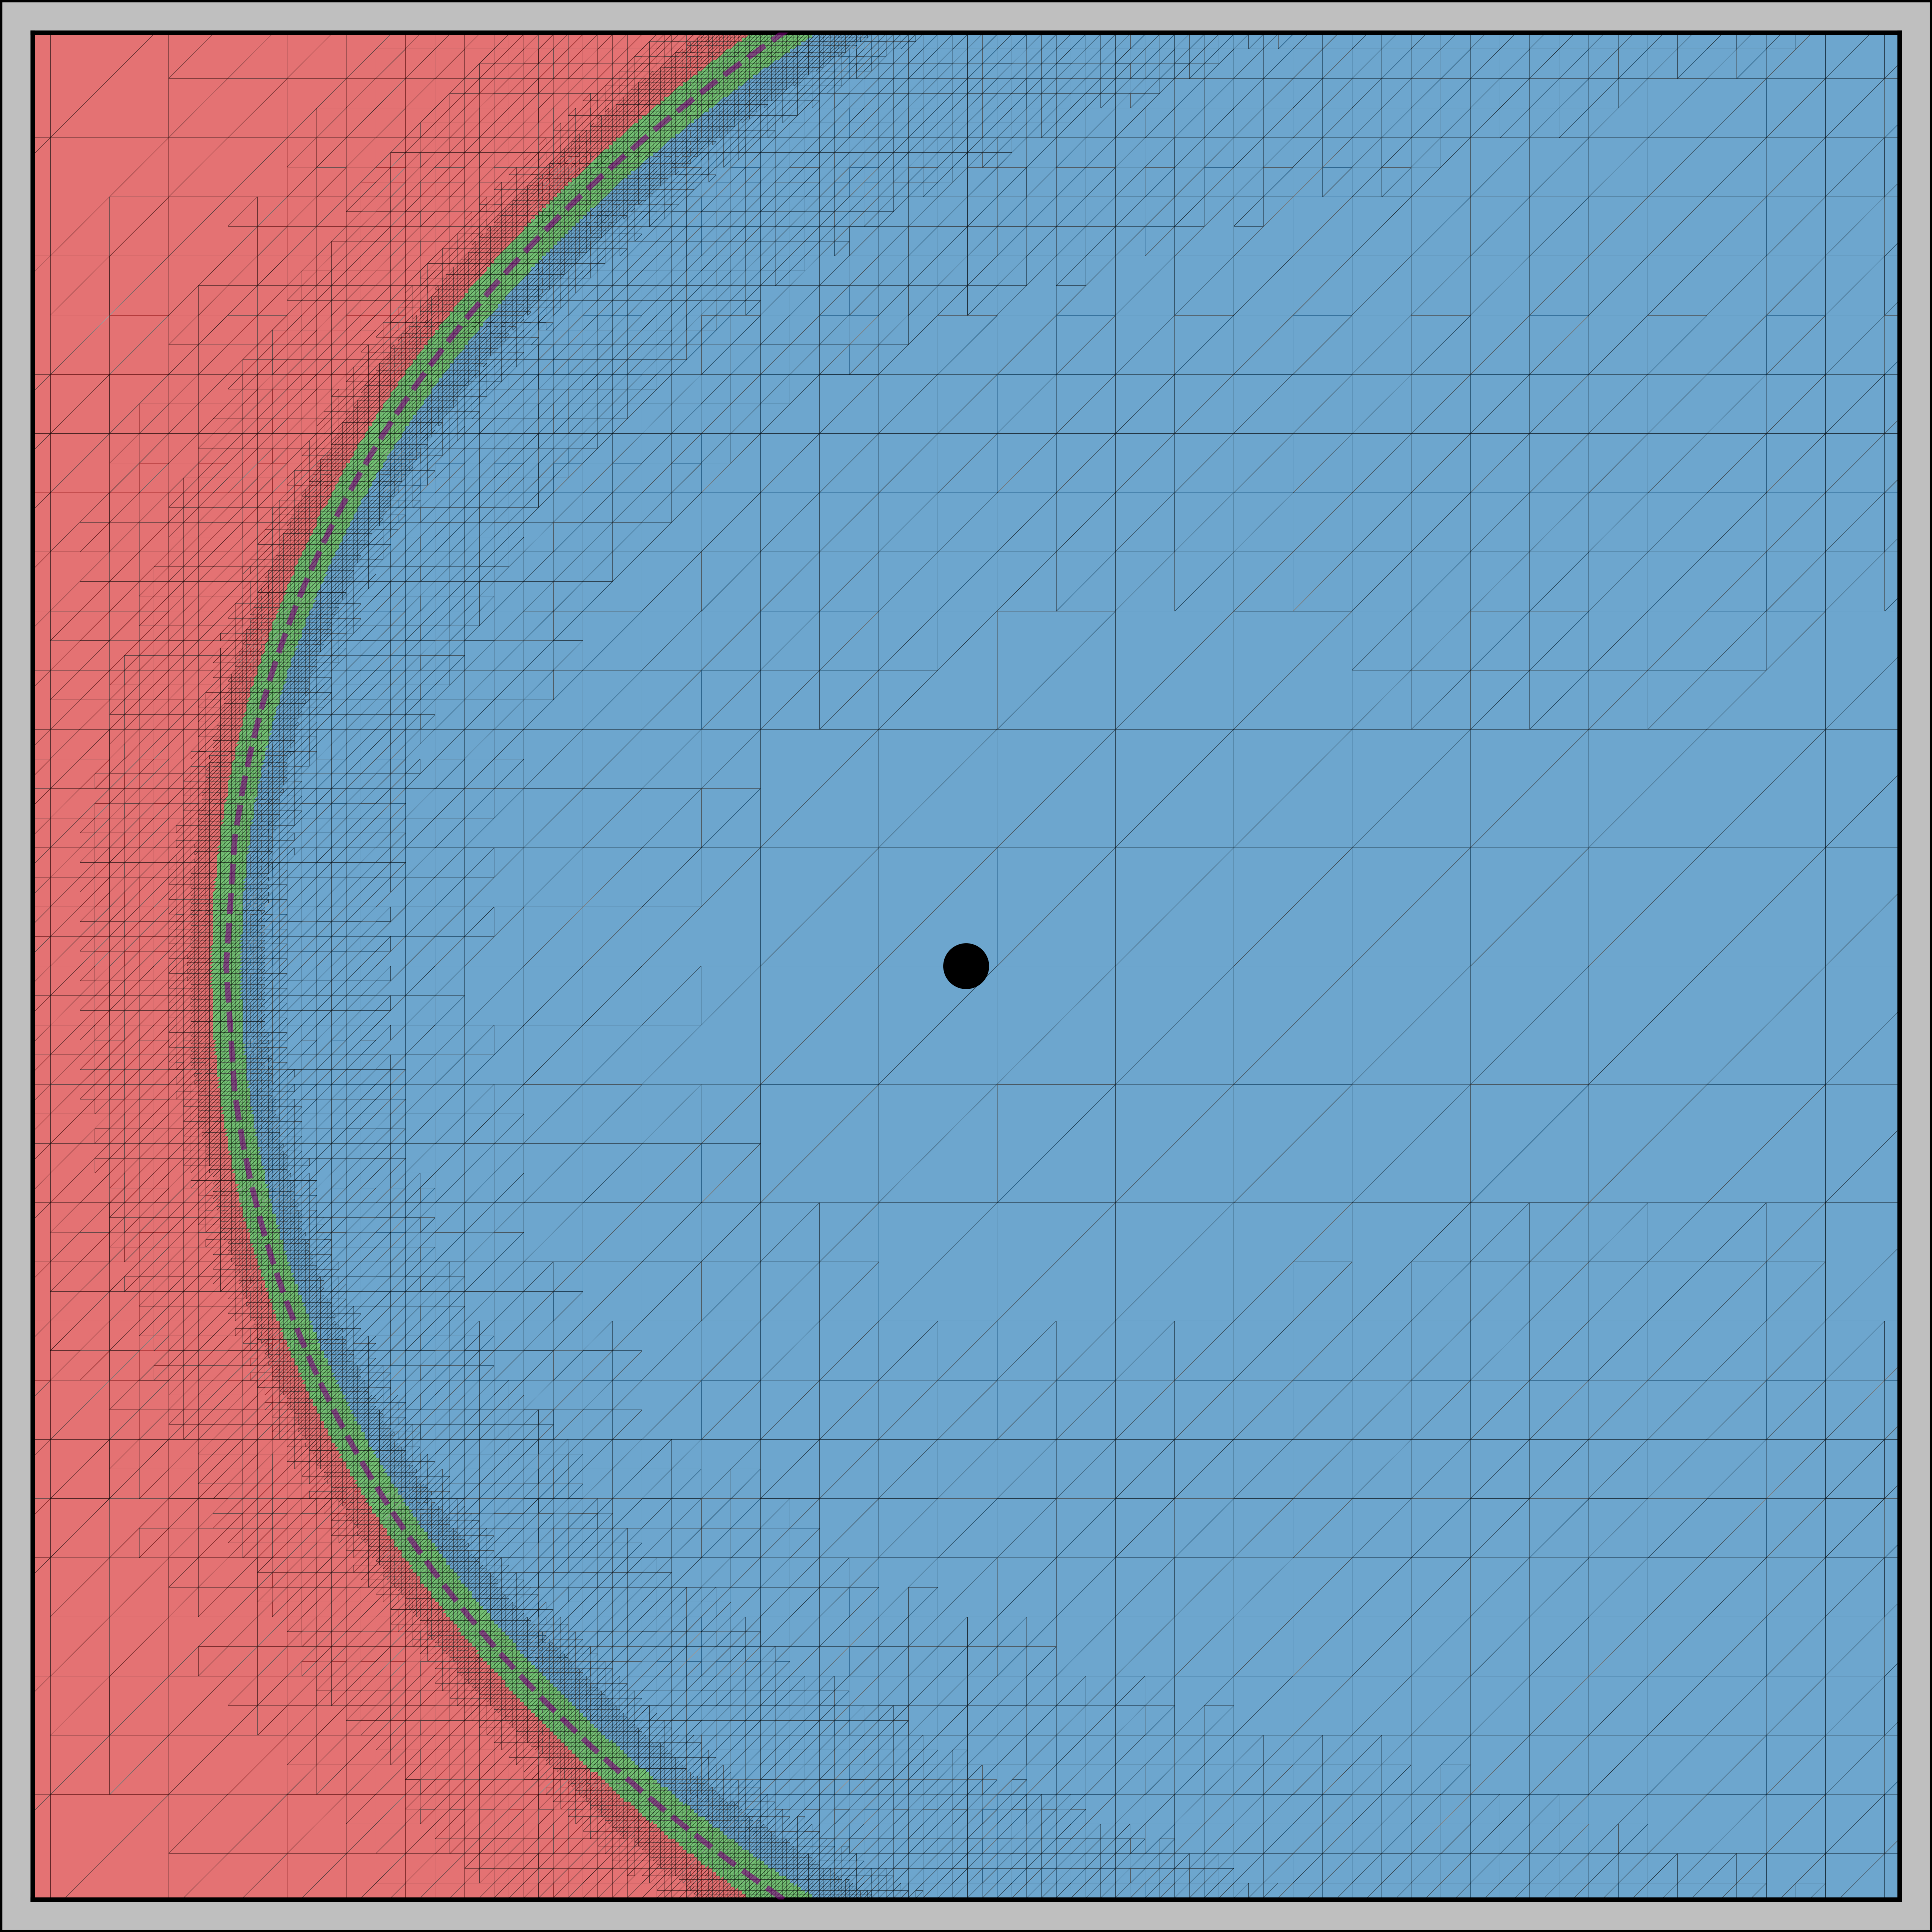
\includegraphics[width=\textwidth]{images/advection_zoom_standalone.png}
%     \end{minipage}
% \label{advectresults}
% \end{figure}


\begin{figure}[htbp]
    \centering

    \includegraphics[width=\textwidth]{images/advection_sweeps_combined.png}

    \vspace{-1.3em}

    \begin{minipage}[t]{0.69\textwidth}
        \setlength{\abovecaptionskip}{0pt}
        \caption[The Computed $\epsilon = 0.5$ Pseudospectral Picture for the One-Dimensional Advection--Diffusion Operator]{
            Outer-refinement levels $k=0,3,7$ for
            \Cref{outerloop} applied to the $\epsilon = 0.5$ pseudospectrum of the
            one-dimensional advection--diffusion operator \eqref{advect}.
            The colour scheme is as in \Cref{dirac results}. The purple dashed curve
            is a reference contour computed using \texttt{Pseudospectra.jl}
            \cite{PseudospectraJL}. A magnified view of the $\mathcal{T}_7$ result, along with the reference contour, 
            over $[1.8,5.1]\times[-1.6,1.6]$ is shown to the right.
        }
        \label{advection results}
    \end{minipage}
    \hfill
    \begin{minipage}[t]{0.28\textwidth}
        \vspace{0pt}
        \centering
        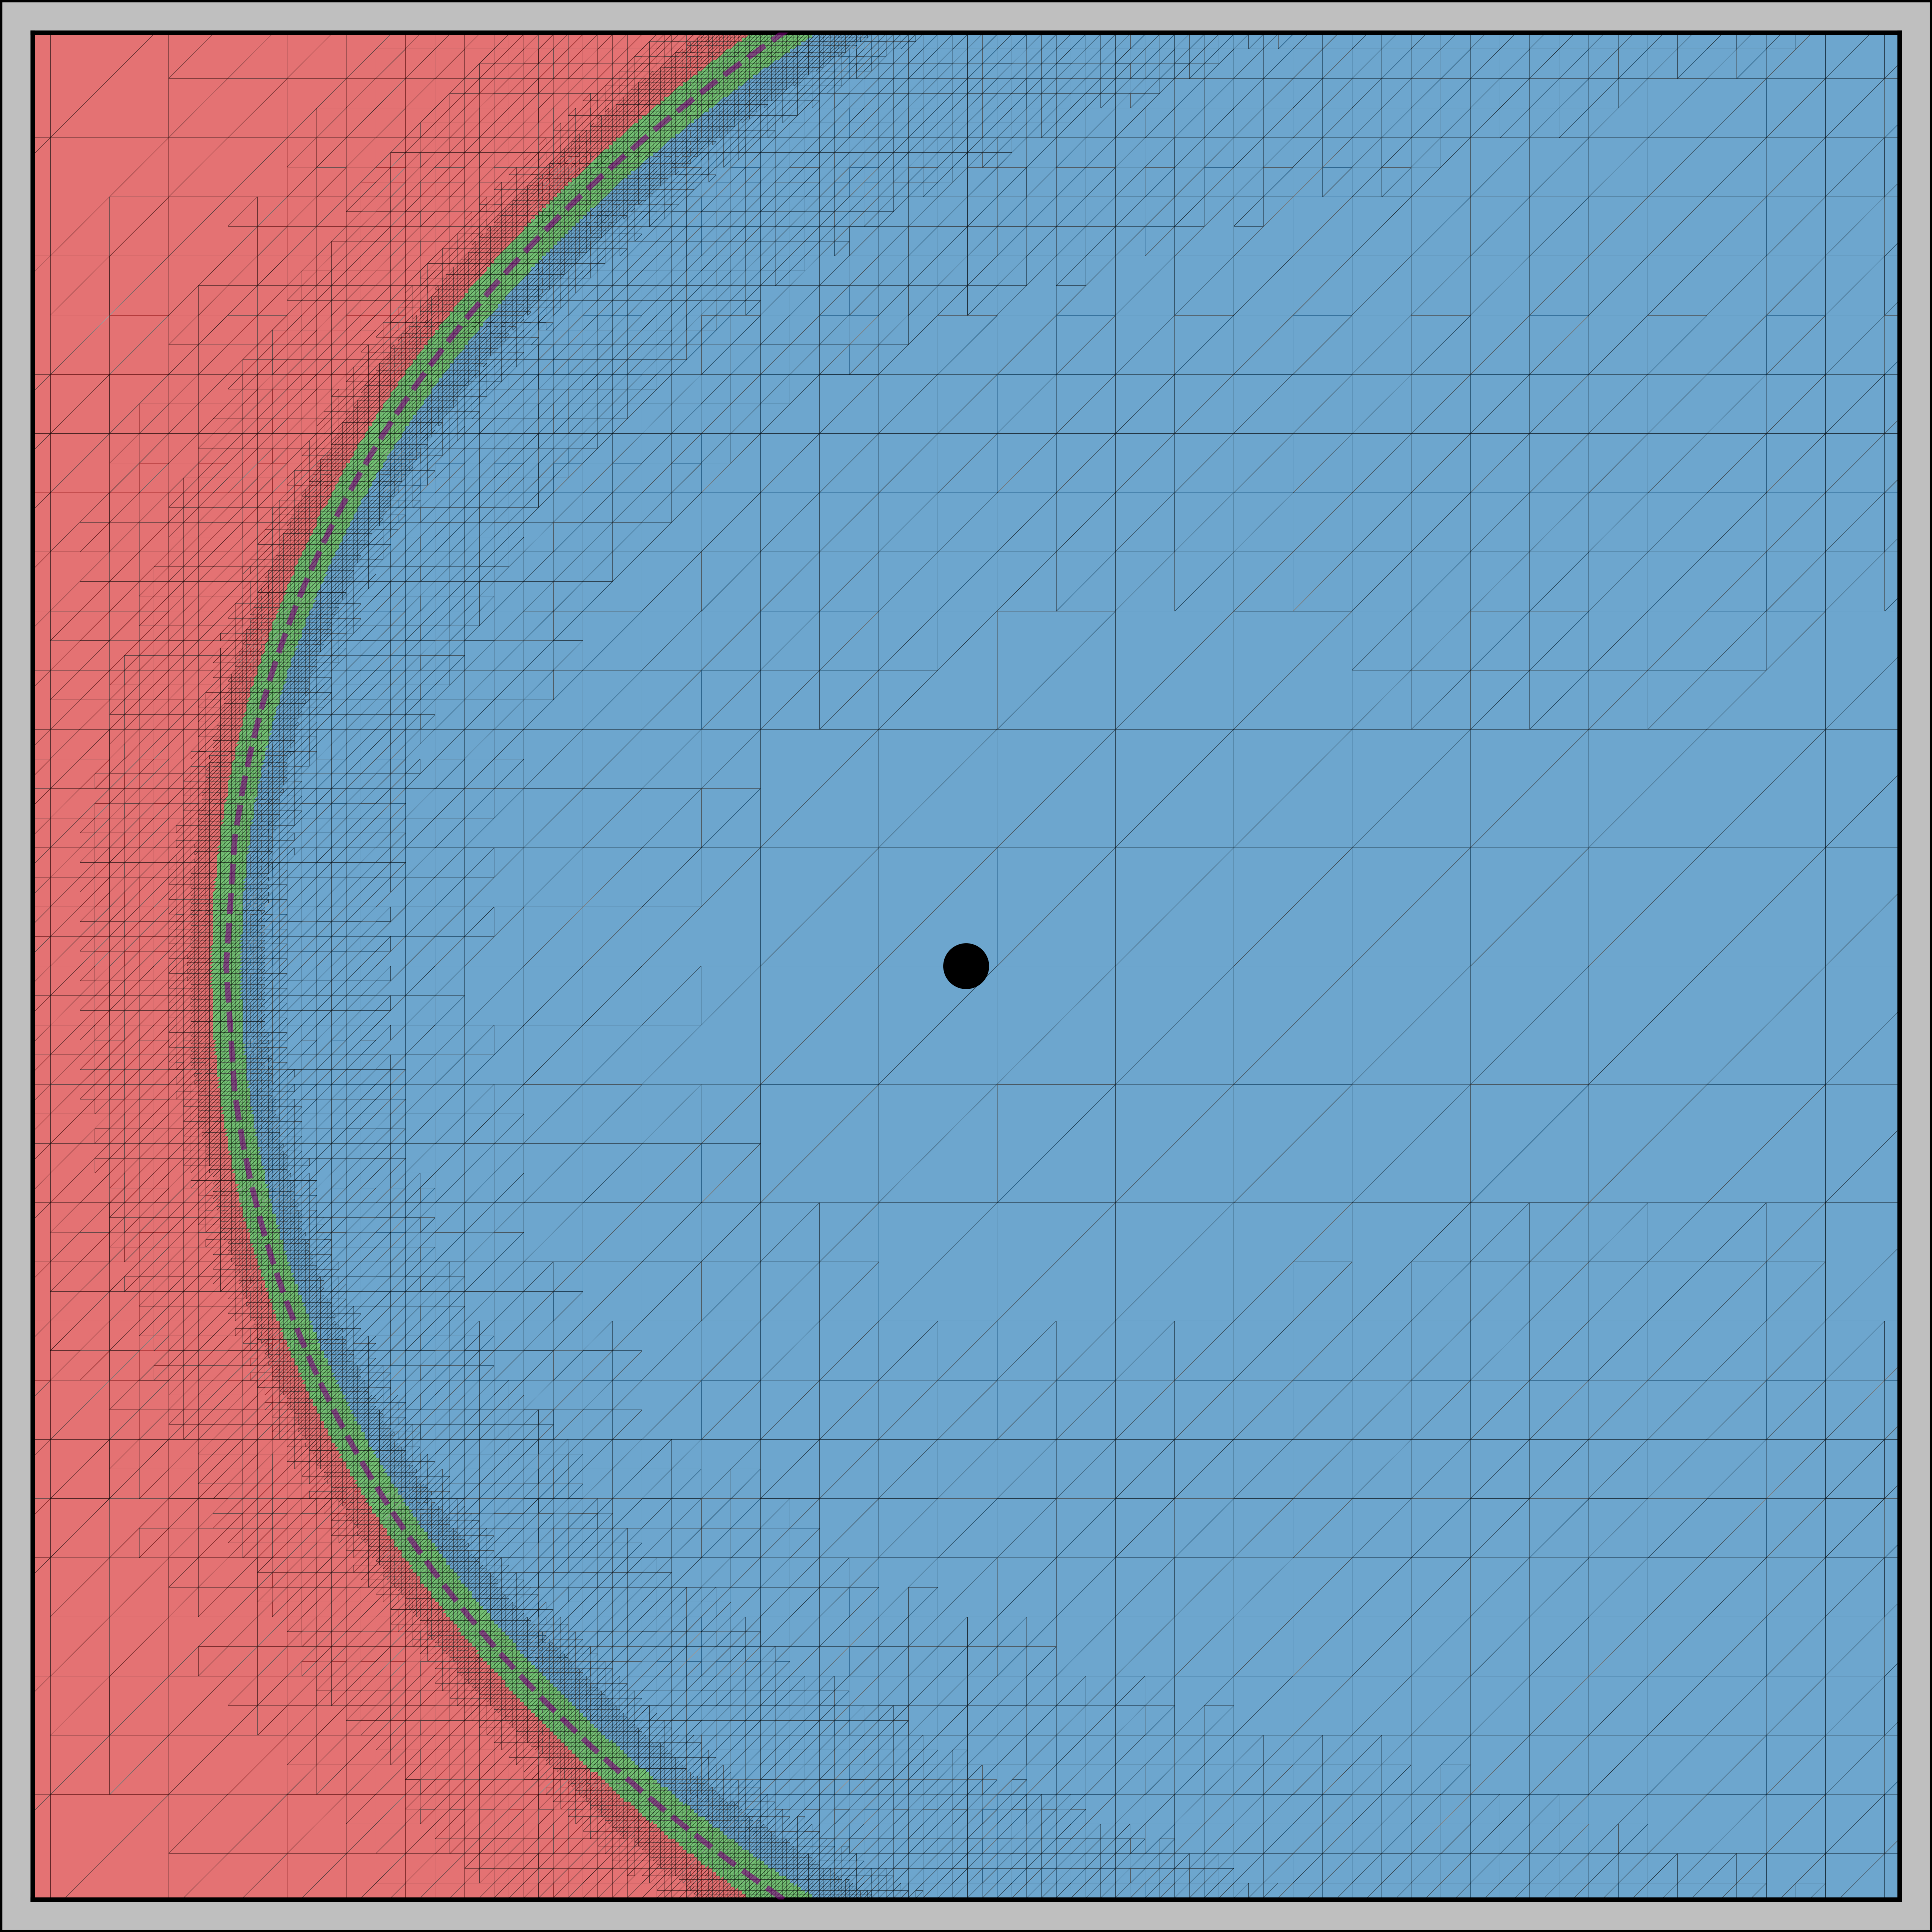
\includegraphics[width=\textwidth]{images/advection_zoom_standalone.png}
    \end{minipage}
\end{figure}